%Abläufe
\section{Abläufe}
\subsection{Frontend}
\subsection{Backend}
Der folgende Prozess zeigt wie das Backend auf die get-Abfrage eines frisch erstellten SingleOnlineLinks reagiert.
Dabei wird eine REST-Anfrage an die im SingleOnlineLink spezifizierte URL gestellt und aus der JSON Response wird das entsprechende Sensorthing gebaut.
Dazu wird über die Javax Klassen Client and Webtarget eine HTTP-Verbindung zur Sensorthings Datenbank aufgebaut und dort der entsprechende Query in Form einer REST-Anfrage ausgeführt.
\begin{center}
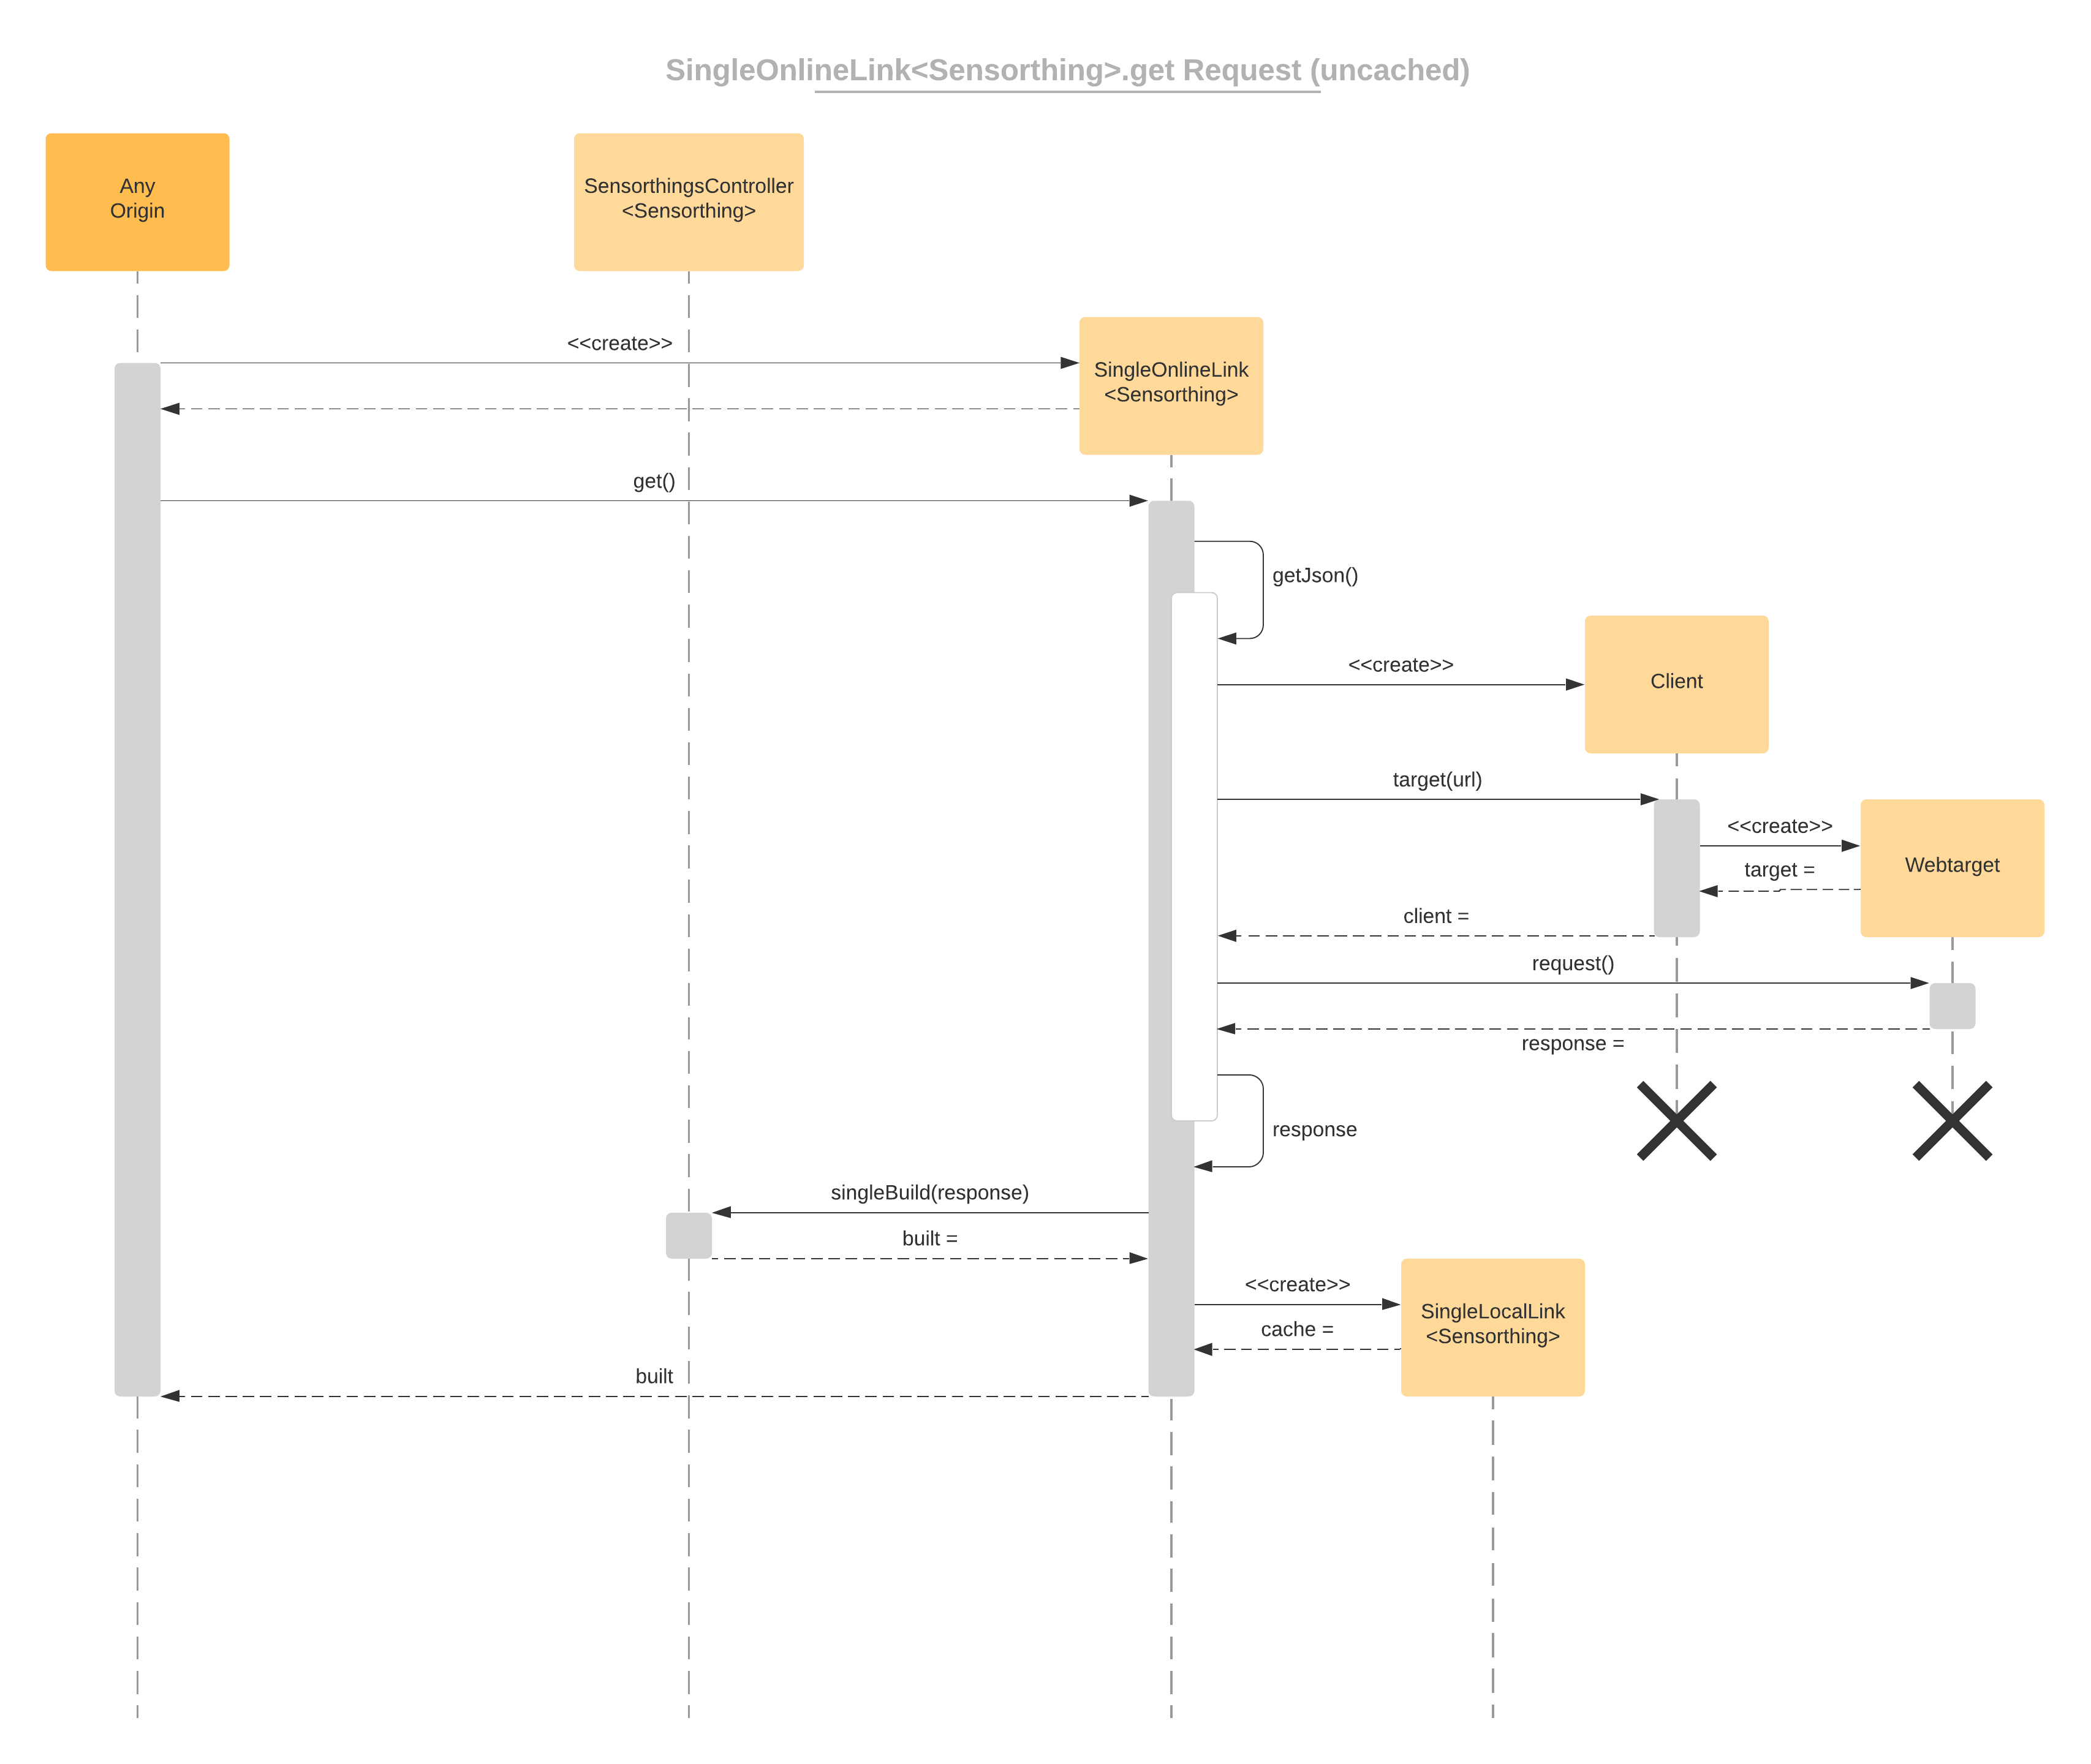
\includegraphics[scale=0.12]{media/backend/processes/SingleOnline.png}\captionof{figure}{Get-Request auf einem SingleOnlineLink}
\end{center}
Dieser Prozess verläuft praktisch analog zu SingleOnlineLink, es wird allerdings ein NavigationLink abgefragt, der mehrere Ergebnisse haben kann.
Dementsprechend wird bei der Konstuktion in \emph{multiBuild()} für die in einem JSON Array zurückgegebenen JSON Objects einzeln die bereits in SingleOnlineLink verwendete \emph{singleBuild()} Funktion aufgerufen.
\begin{center}
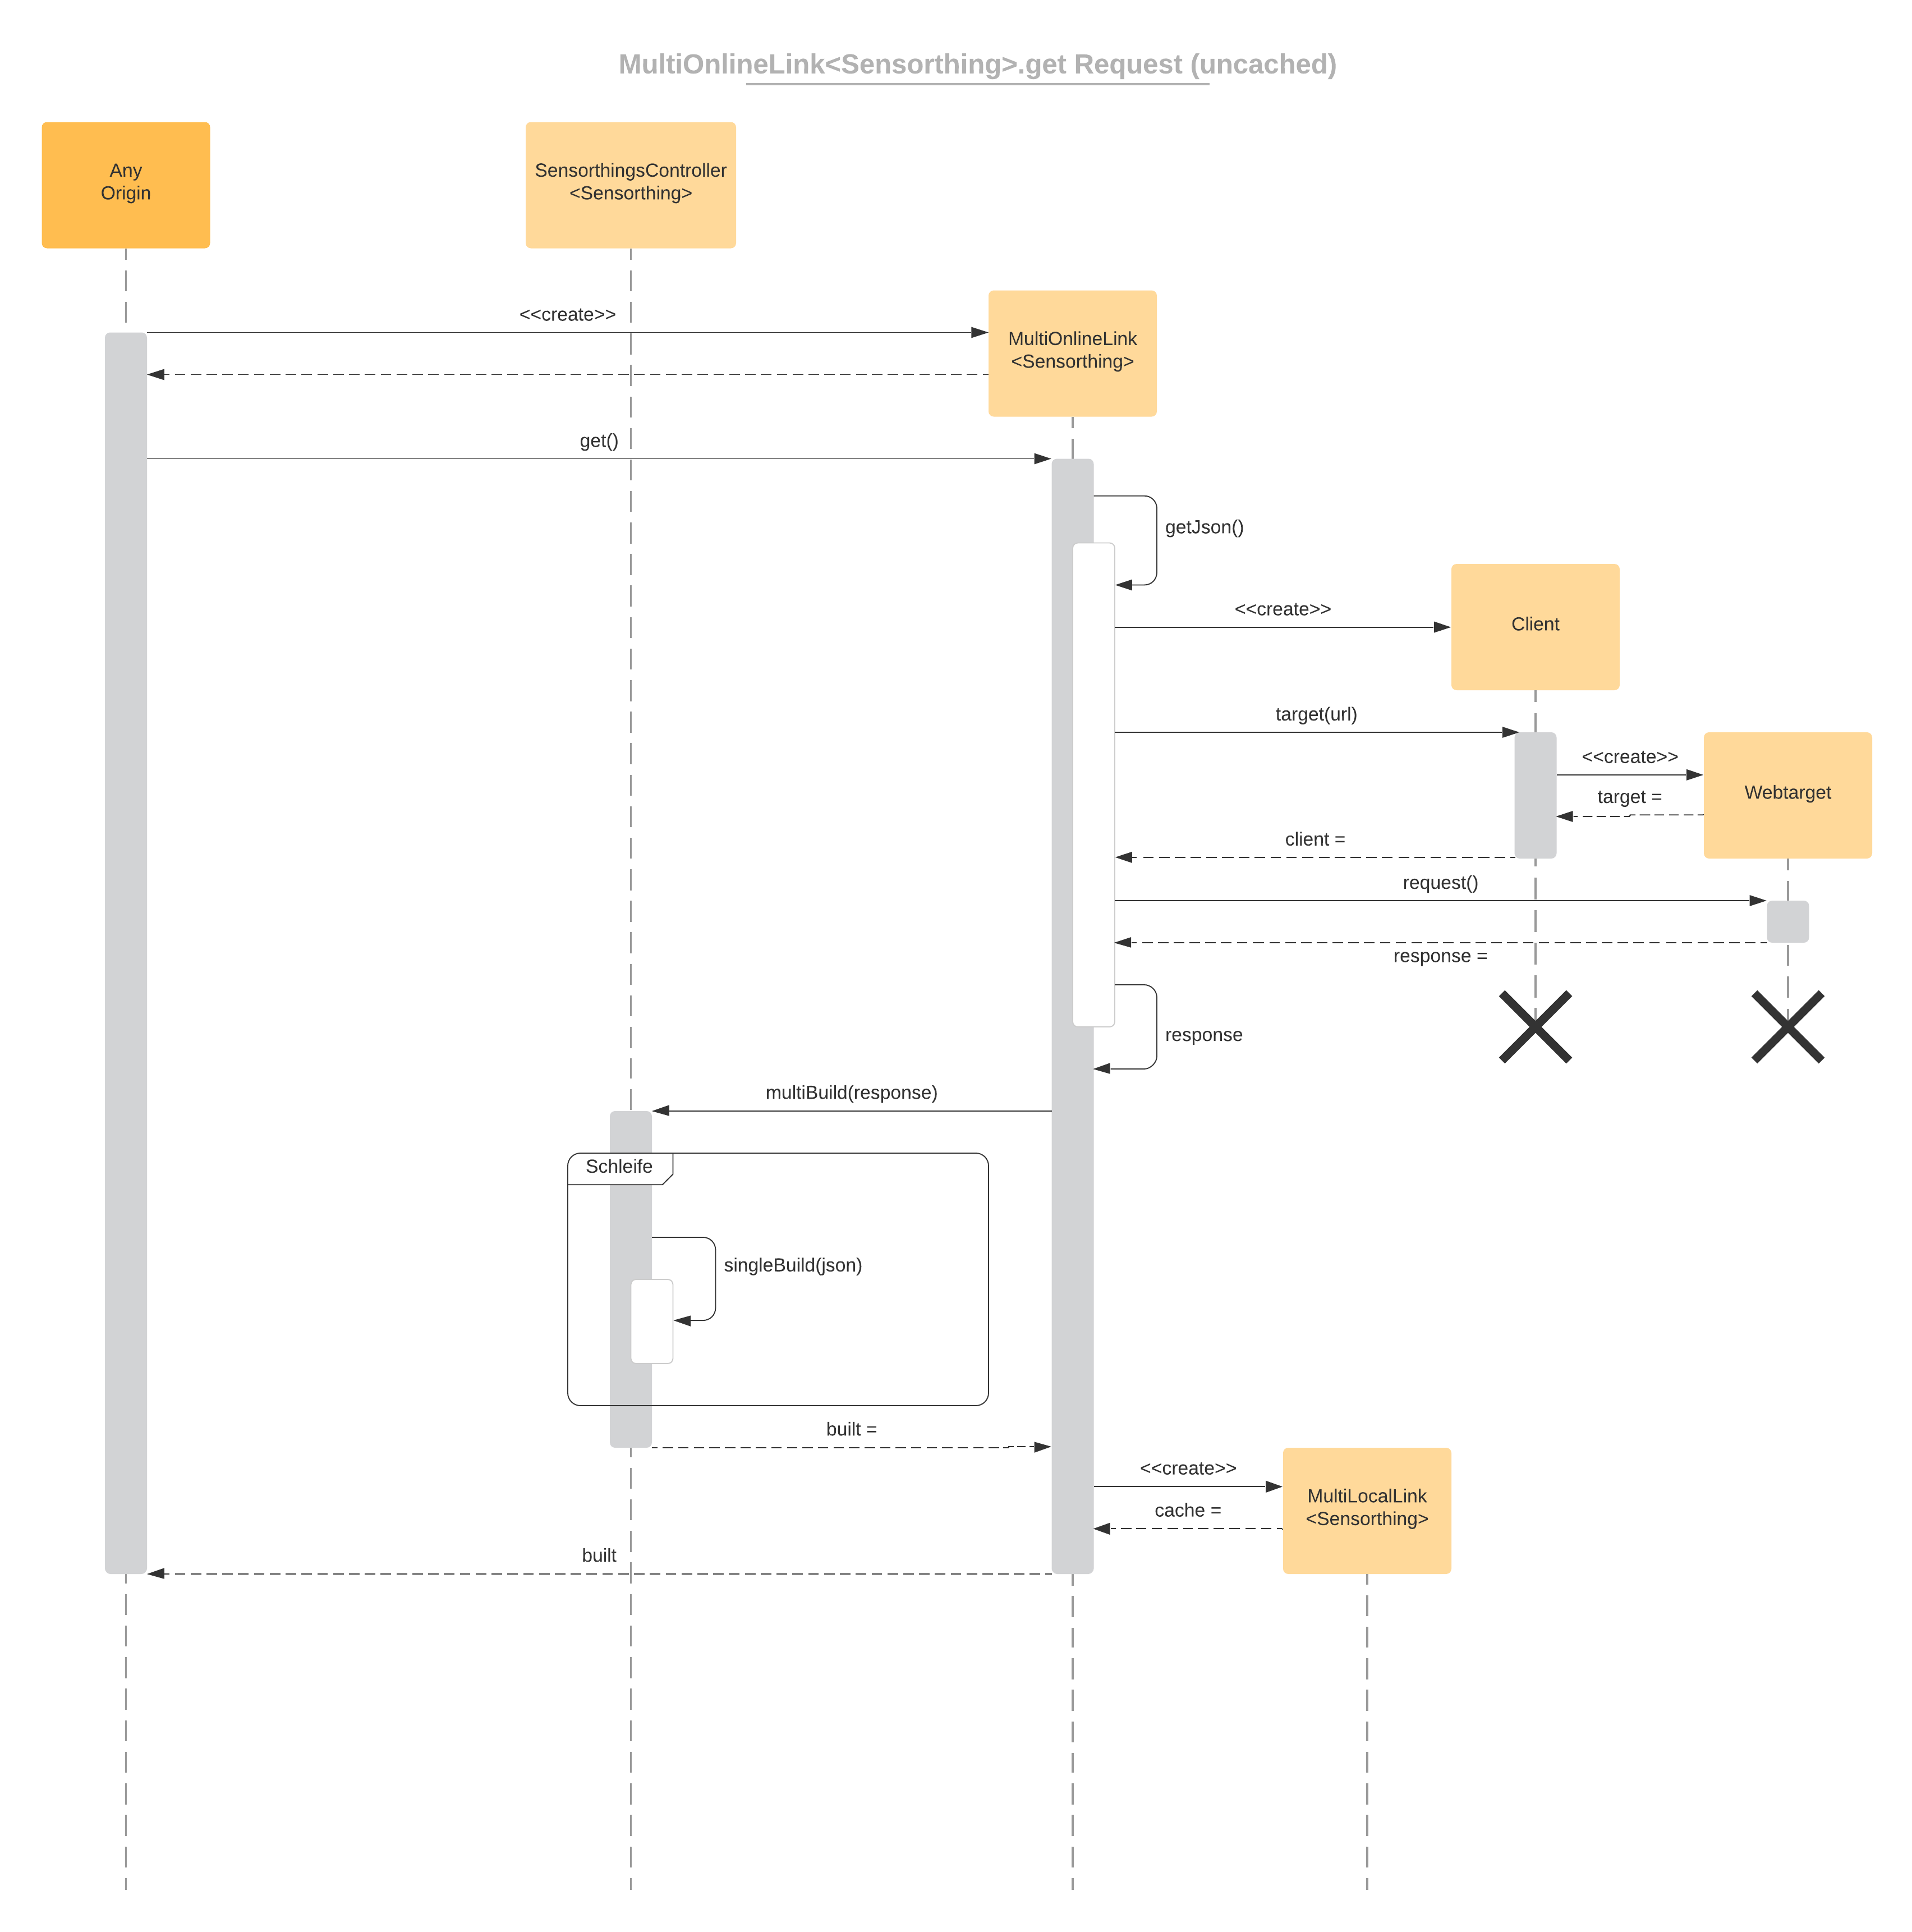
\includegraphics[scale=0.12]{media/backend/processes/MultiOnline.png}\captionof{figure}{Get-Request auf einem MultiOnlineLink}
\end{center}
Während es sich bei den vorherigen Prozessen um den Verlauf bei nicht-gecachten frischen NavigationLinks handelt, werden im folgenden SingleLocalLink und MultiLocalLink betrachtet,
die das Ergebnis der mit Ihnen verbundenen REST-Abfrage bereits gecached haben. Solche Links entstehen im Programmverlauf natürlich, da jede nicht-gecachte Get-Request ein lokales Caching in einem neuen LocalLink zur Folge hat.
Diese Links beschleunigen also bei mehrfach Verwendung des selben Links die Anfrage Geschwindigkeit erheblich, da keine Kommunikation mit der Sensorthings Datenbank erforderlich ist.
\begin{center}
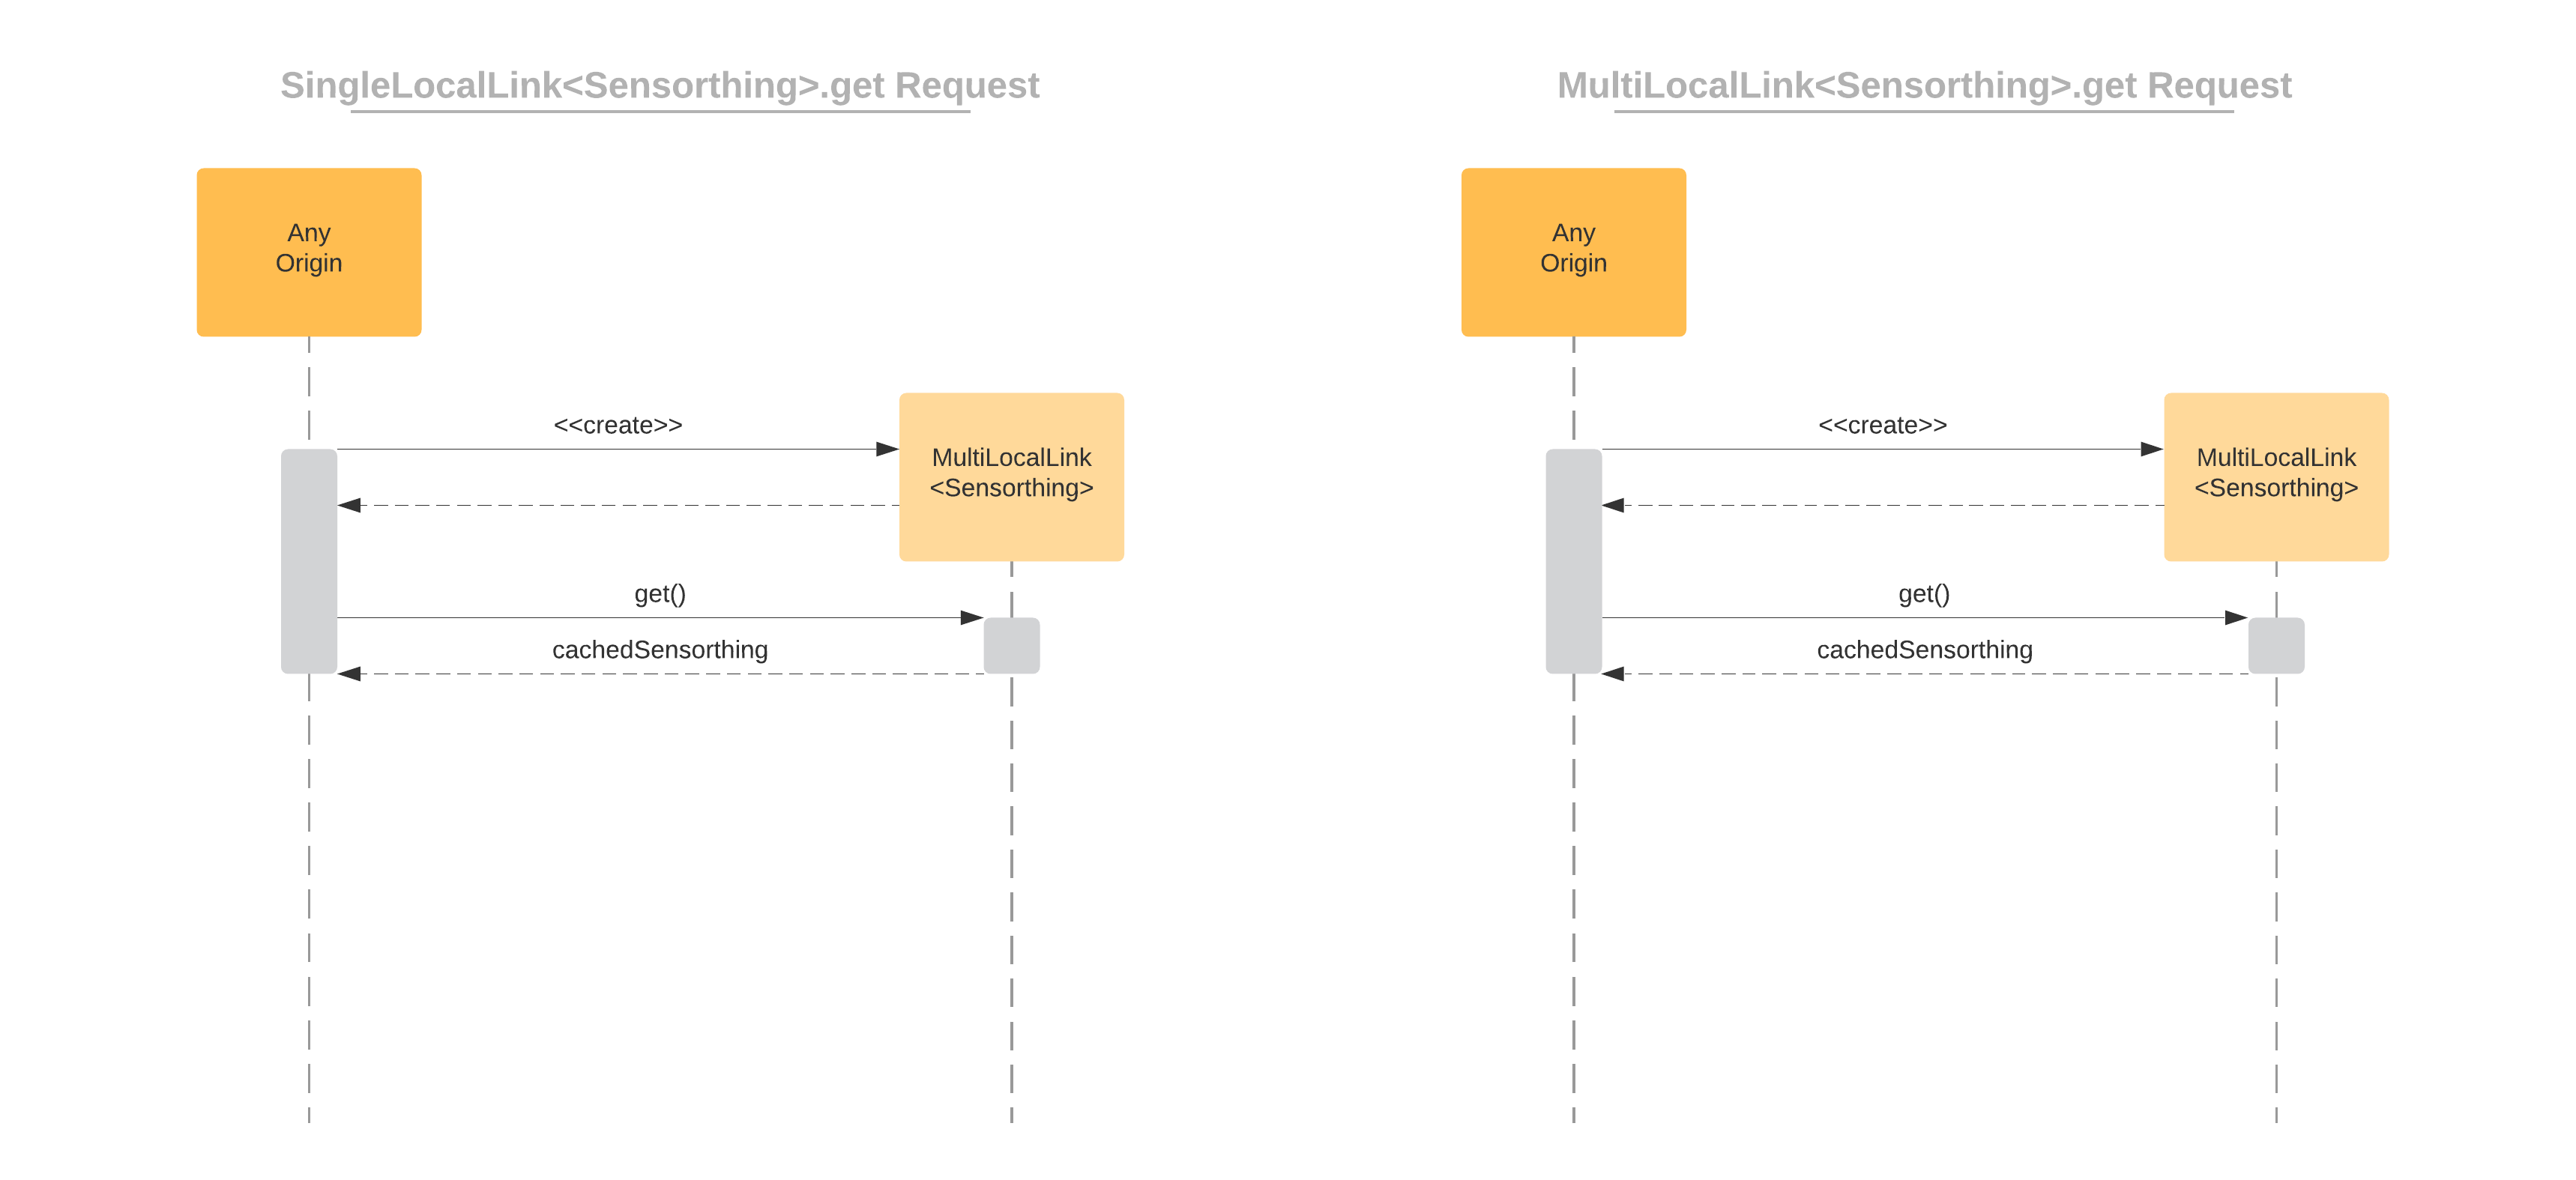
\includegraphics[scale=0.12]{media/backend/processes/SingleAndMultiLocal.png}\captionof{figure}{Get-Request auf einem Single-/MultiLocalLink}
\end{center}
Dieser Prozess zeigt die Hauptschnittstelle zwischen Frontend und Backend, dabei wird grob zwischen den zwei Abfragearten get und getAll unterschieden, die sich in unterschiedlichem Mapping und der Kardinalität ihrer Rückgabe äußern.
Get gibt dabei ein einzelnes Sensorthing Entity zurück, das den in POST-Parametern spezifizierten Anforderungen genügt, wobei getAll eine Menge von Sensorthings Entities zurückgibt, den Anforderungen entsprechen.
Aufgrund des Entwurfs mit generischen Typen und der Verwendung von Spring, ist der Prozess im Grunde unabhängig von dem konkreten Sensorthings Model durchführbar.
Die Auswahl eines bestimmten Models findet dabei über das Mapping statt, während die Anforderungen in den POST-Parametern enthalten sind und von Spring die kompatible Methode ausgesucht wird.
Der Prozess ist simpel: Spring dekodiert die POST-Anfrage, die kompatible Funktion erstellt den passenden Query als neuen NavigationLink und startet eine Get-Request.
\begin{center}
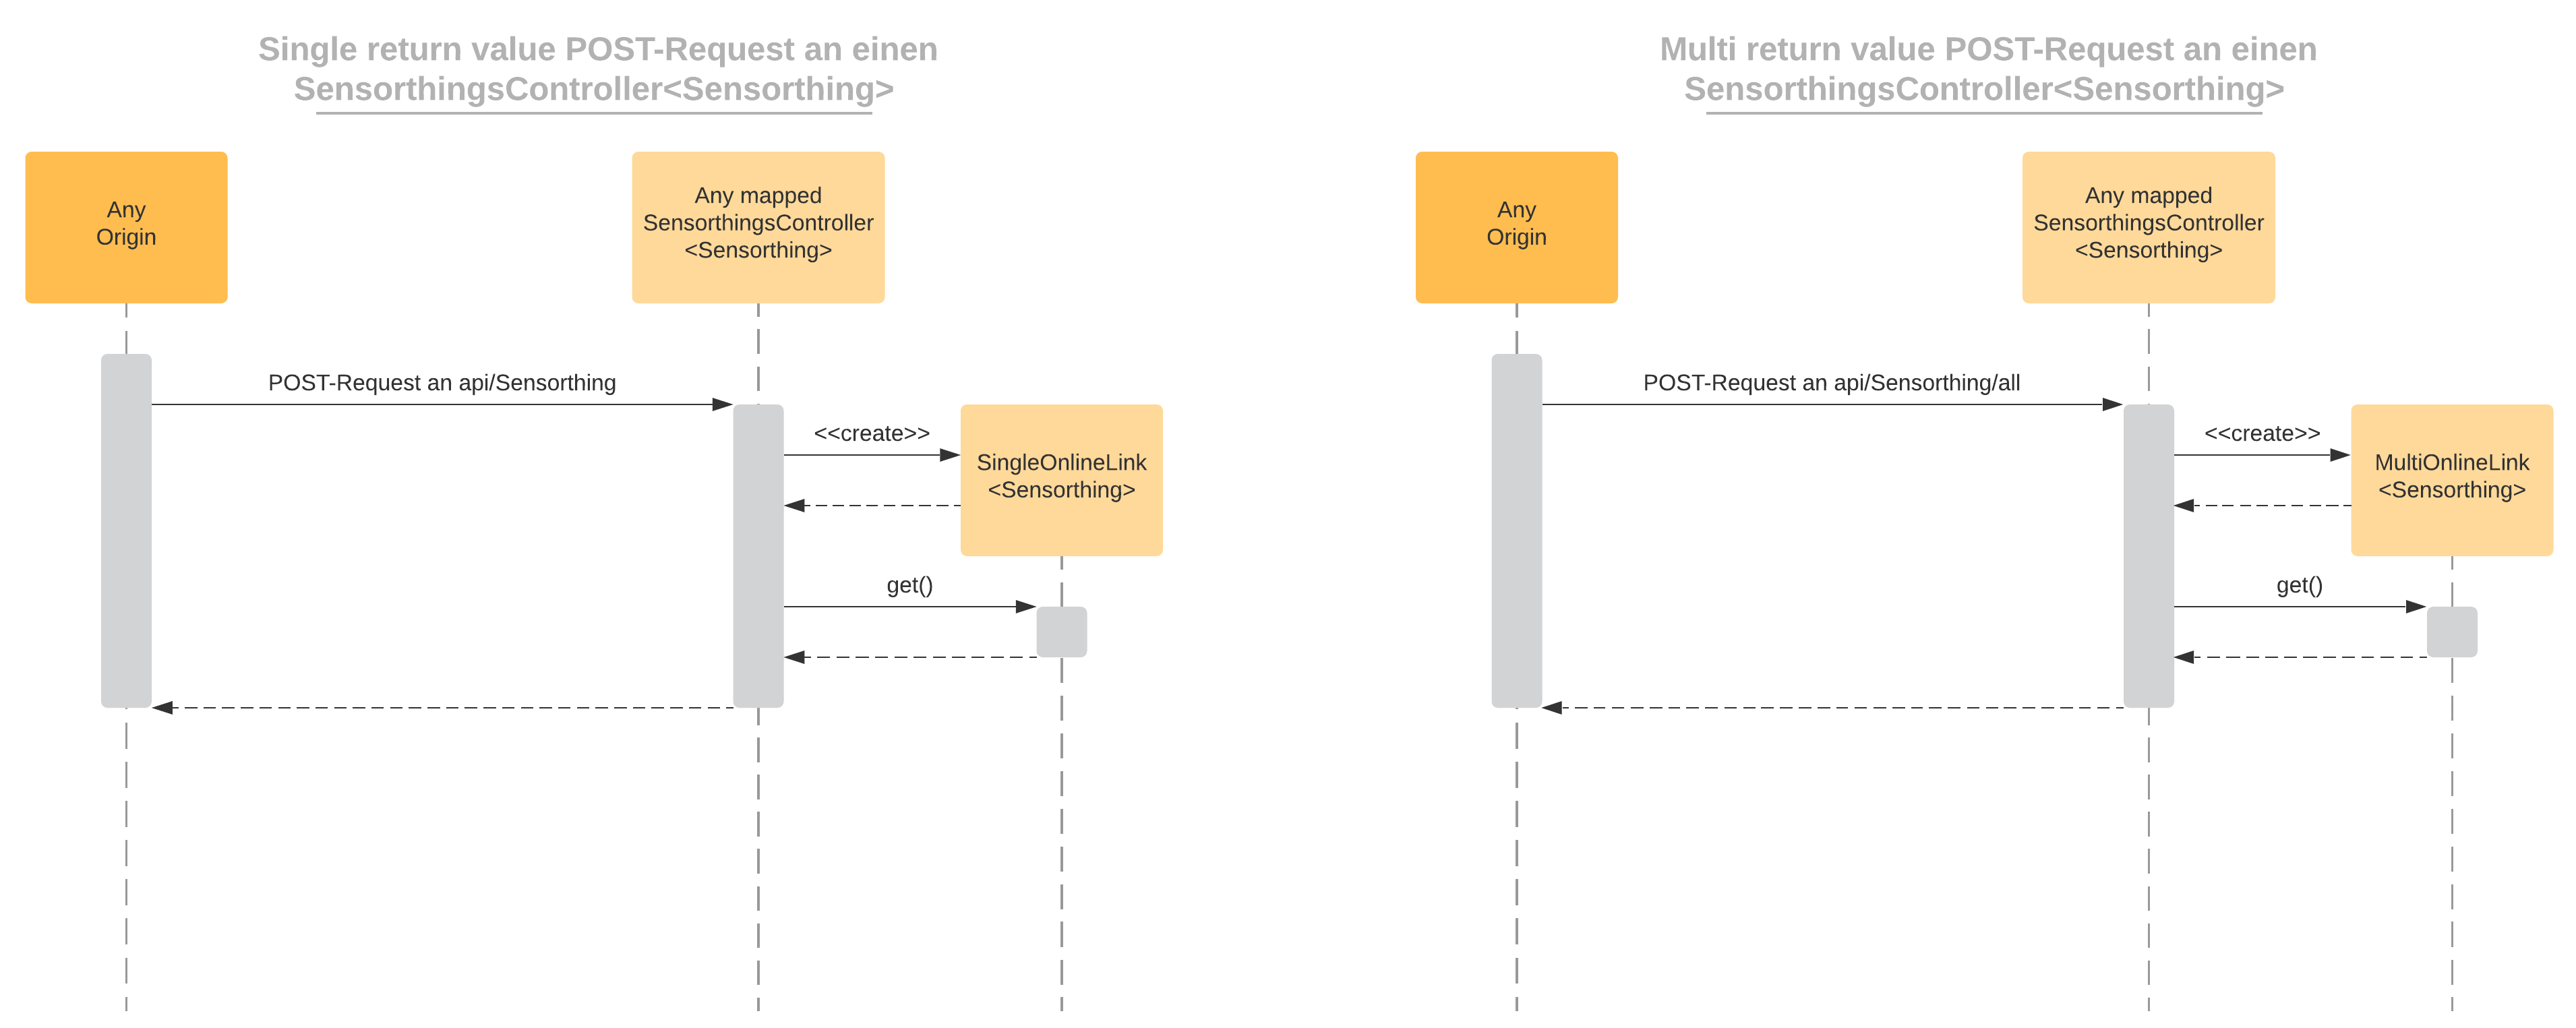
\includegraphics[scale=0.12]{media/backend/processes/SingleAndMultiReturnPost.png}\captionof{figure}{SensorthingsController POST-Request mit JSON Response}
\end{center}
Der Prozess der Interpolation funktioniert ähnlich wie der Prozess zuvor. Die benötigten Parameter werden als POST-Parameter übergeben, von Spring aufgeschlüsselt und auf die Funktion angewandt. Die konkret gewählte Interpolationimplementierung, in diesem Fall BarnesInterpolation,
berechnet dann auf diesen Parametern die Interpolation und gibt dies zurück.
\begin{center}
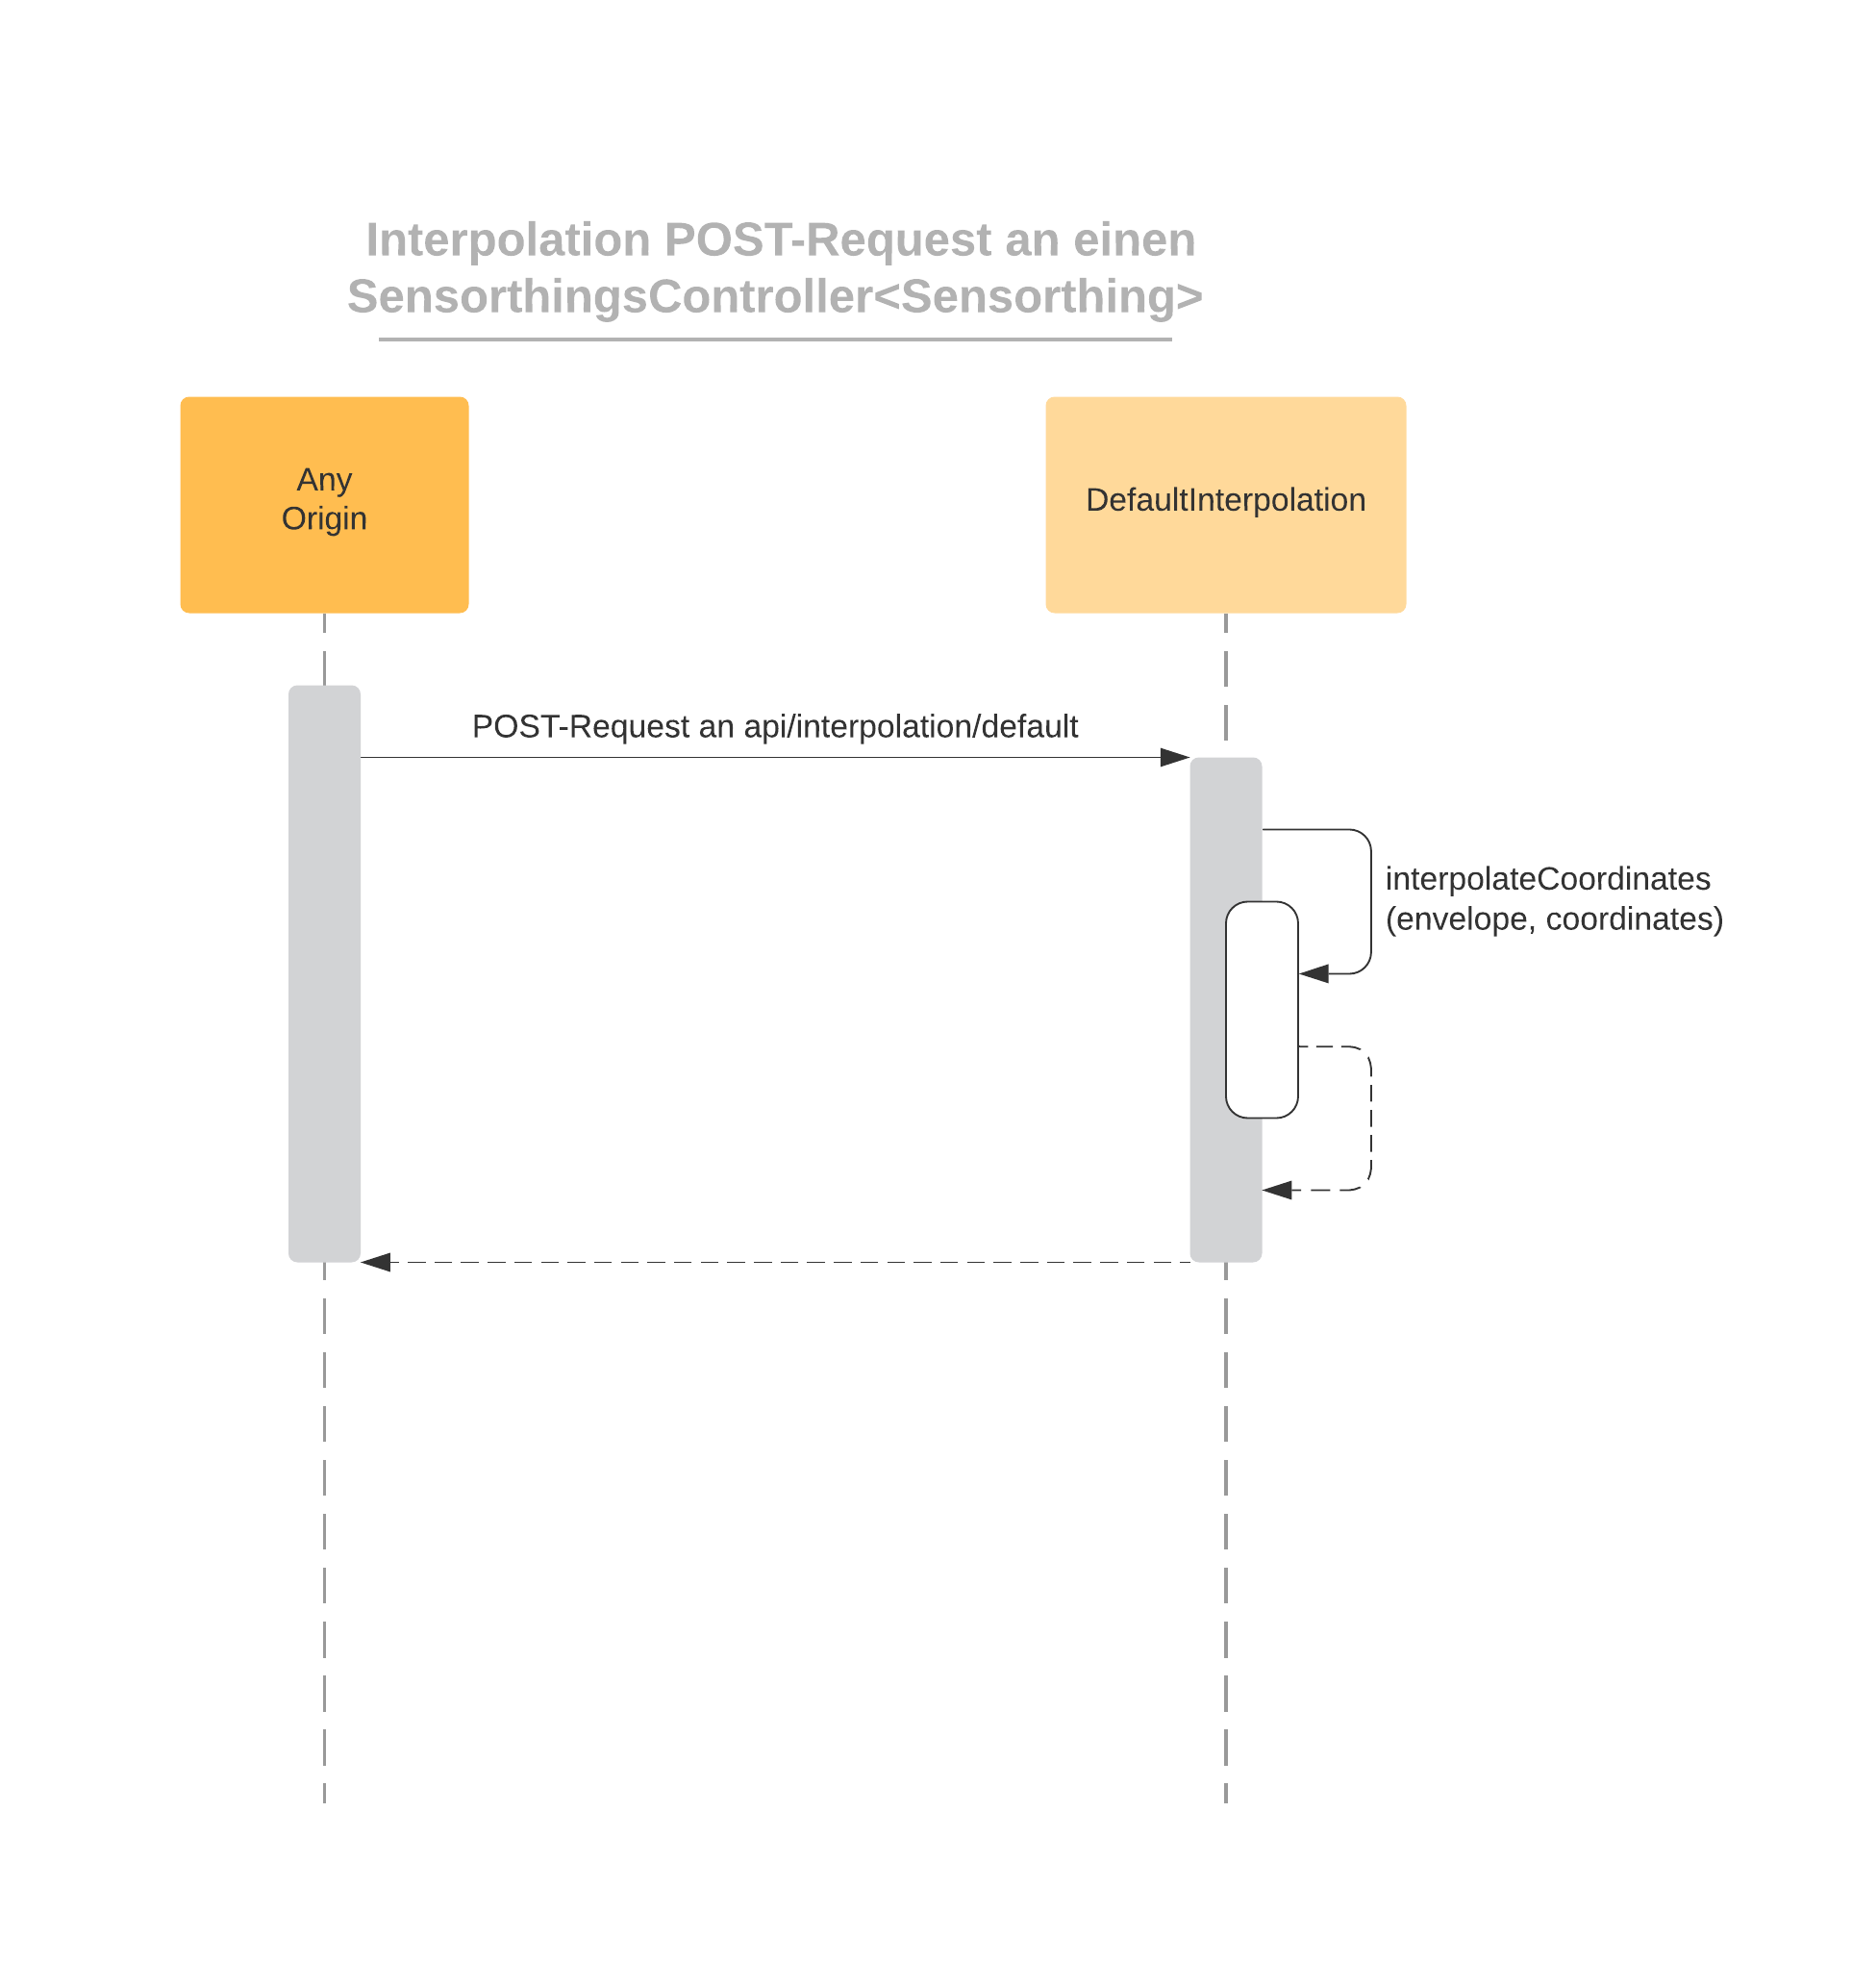
\includegraphics[scale=0.12]{media/backend/processes/Interpolation.png}\captionof{figure}{Interpolation POST-Request mit interpolierten Daten als JSON Response}
\end{center}
